% !TeX root = main.tex
\chapter{Performance of colourised waveforms}\label{chp:colourised}

In Chapter~\ref{chp:background}, we saw that waveforms do not convey much information about the audio content and are
very difficult to read without an expert understanding.
Despite this, waveforms continue to be the most popular interface for interacting with audio content.
Given that there are no signs that waveforms will stop being the most widely used audio visualisation, we are
interested in finding out whether something can be done to improve them.

The user group we chose for this study is radio producers, as this is the overall focus of our research.
It is quite common for radio programmes to be released as podcasts after broadcast.
Music licensing rules require that music is not included in podcasts, so in order to release a radio programme as a
podcast, producers must remove the music from the programme.
This is a tedious and time-consuming task.

We also saw in Chapter~\ref{chp:background} that advances in audio analysis, data visualization and understanding of
cross-modal links mean it is possible to develop audio visualizations that better reflect what people are hearing so
that users can navigate and edit with ease, and be more productive.
We are interested in exploring how these approached could be used to create an enhancing waveform visualisation that
assist producers in performing this task.

Radio producers have been using waveforms for many years and have developed the expert skills required to be able to
read them.
Adding colour to waveforms allow us to include extra information while being able to retain a familiar interface that
they can already read.

%\section{Background}

%% WAVEFORM NAVIGATION
%Lots of studies have considered the performance of waveforms for audio navigation, and there are numerous other
%visualisations that perform better.
%However they all use waveforms as the baseline and have not actually measured the performance of the waveform itself.

%% SPEECH/MUSIC DISCRIMINATION
%SMD algorithms all follow the same general approach.
%Raw metric generated, segmented, then clustered.
%Humans are very good at pattern recognition, so by presenting the raw information they may be able to interpret the
%data better than the automated segmenting/clustering.

\section{Methodology}

In this study we aimed to evaluate how audio visualisations affect user performance.  We did this by conducting an
experiment in which participants performed a simple task using different audio visualisations.

% The task
For the task, we chose segmentation of music from speech.  We wanted the task to be a common radio production activity,
but one that is simple enough that it can be performed by anybody.  In radio production, music has to be removed when
editing an off-air programme recording into a podcast, due to music rights issues. The amplitude profile displayed by
the audio waveform can be used to distinguish between music and speech, but at typical zoom levels, it is not obvious.

% Conditions
\subsection{Conditions}
We chose to use the following conditions for the audio visualisations. An example of each condition is shown in
Figure~\ref{fig:conditions}.

\begin{enumerate}[label=C\arabic*.]
  \item \textbf{None}: No visualisation, audio only.
  \item \textbf{Waveform}: Audio waveform in a single colour.
  \item \textbf{Enhanced}: Audio waveform with colour mapped to low energy ratio.
\end{enumerate}

\begin{figure}[ht]
  \centering
  \begin{subfigure}{.3\textwidth}
    \centering
    \includegraphics[width=\columnwidth]{figs/condition1.png}
    \caption{C1: None}
  \end{subfigure}
  \begin{subfigure}{.3\textwidth}
    \centering
    \includegraphics[width=\columnwidth]{figs/condition2.png}
    \caption{C2: Waveform}
  \end{subfigure}
  \begin{subfigure}{.3\textwidth}
    \centering
    \includegraphics[width=\columnwidth]{figs/condition3.png}
    \caption{C3: Enhanced}
  \end{subfigure}
  \caption{The audio visualisation conditions we tested.}
  \label{fig:conditions}
\end{figure}

% Listening
We included a condition in which there was no visualisation, as we were interested in using it as a baseline to measure
the performance of the normal waveform. For this condition, the participant must rely purely on listening to the audio.
For the other two conditions, they are able to both listen and use the visualisation.

% SMD
For the enhanced visualisation, we extracted an audio feature that was relevant to the task and mapped it to the colour
of the waveform.
Speech/music discrimination (SMD) is a research topic that aims to automatically segment speech and music.  These
systems are often targeted at recordings of radio broadcasts
\citep{Goodwin2004,Wieser2014,Saunders1996,Pikrakis2008,Pikrakis2006a}. In general, SMD systems extract several audio
features, then use clustering techniques to group those features into segments of either speech or music.
%Clustering is a task in which comes naturally to humans, but machines often struggle with.

% choosing a feature
We wanted to select a single, one-dimensional (scalar) feature that would help the participant perform their task.
%\citet{Carey1999} found that, other than cepstral features, amplitude-based features performed best.
Low energy ratio (LER, also known as `silent interval frequency', `energy contour dip' and `low short-term energy
ratio') is the frequency in which the energy of a signal falls below a threshold. This simple but effective feature
exploits the fact that speech has frequent silent gaps between words, whereas music does not.  \citet{Panagiotakis2005}
found that on its own, LER can classify 50\% of music segments.

% calculating the feature
We calculated the low energy ratio by extracting the RMS energy (20ms frames, no overlap) and counting the proportion
of frames which fell below a threshold.  The threshold can be set as a fixed value \citep{Liang2005,Panagiotakis2005},
a function of the moving average \citep{Ericsson2009}, or a function of the moving peak value \citep{Saunders1996}.
After empirically testing a variety of radio programme recordings, we chose the latter and configured our threshold as
the third percentile of RMS energy in a one second sliding window.

%Metric does not return perfect results, so user must interpret them

%music tonality \citep{Sell2014}
%energy density analysis \citep{Kacprzak2013}
%??? \citep{Goodwin2004}
%application to TV \citep{Seyerlehner2007}

% mapping the feature
We coloured the waveform by mapping the low energy ratio to a gradient between two easily distinguished colours.  We
used blue to represent speech and pink to represent music.  We chose blue to match the colour of the waveforms in the
BBC's radio production system, and the inverse of its colour, pink.

\subsection{Hypotheses}

We were interested in testing the effectiveness of audio visualisation for navigating and editing audio content. In
particular, we wanted to examine the following hypotheses:

\newcommand{\subscript}[2]{$#1 _ #2$}
\begin{enumerate}[label=H\arabic*.]
  \item \textbf{Effort}: Audio visualisation affects the effort required to segment music from speech, in
    decreasing order of C1, C2 and C3.
  \item \textbf{Time}: Audio visualisation affects the time taken to segment music from speech, in decreasing
    order of C1, C2 and C3.
  \item \textbf{Accuracy}: Audio visualisation affects the accuracy of segmenting music from speech, in
    increasing order of C1, C2 and C3.
    %\item The audio visualisation affects the reported task load, in decreasing order of C1, C2 and C3.
\end{enumerate}

\subsection{Metrics}

Our audio segmentation task involves finding the target audio (in this case, music) and marking the start and end of
the desired region. The two primary activities involved in this are seeking through the audio (by clicking on the
visualisation), and marking the segment (using the buttons or sliders). To measure effort, we counted the number of
seek actions used to complete the task.

To measure time, we calculated how long it took to complete each task. To avoid including `downtime' at the start and
end of the task, we calculated the task completion time as the difference between the first user action (e.g.
play/seek/mark) and the last mark action.

For accuracy, we measured the error of the result. We calculated this by using ground truth data about the precise
start and end time of the music in the audio, then finding the sum of the absolute error of the selected in-point and
out-point.

In addition to the above metrics, we included a questionnaire to gather perceptual data about the task. For this, we
used the NASA Task Load Index, or `NASA-TLX', \citep{Hart1988} questions, listed below. Responses are captured using on
a scale between -10 and 10 with the following labels.

%\begin{table}[ht]
  %\begin{center}
    %{\small
    %\begin{tabular}{l l l l}
      %\hline
      %Mental demand & How mentally demanding was the task? & very low & very high \\
      %Physical demand & How physically demanding was the task? & very low & very high \\
      %Temporal demand & How hurried or rushed was the pace of the task? & very low & very high \\
      %Performance & How successful were you in accomplishing what you were asked to do? & perfect & failure \\
      %Effort & How hard did you have to work to accomplish your level of performance? & very low & very high \\
      %Frustration & How insecure, discouraged, irritated, stressed, and annoyed were you? & very low & very high \\
      %\hline
    %\end{tabular}
  %}
  %\end{center}
  %\caption{NASA Task Load Index metrics}\
  %\label{tab:nasatlx}
%\end{table}

{\singlespacing
\begin{itemize}
  \item Mental demand -- How mentally demanding was the task? [very low/very high]
  \item Physical demand -- How physically demanding was the task? [very low/very high]
  \item Temporal demand -- How hurried or rushed was the pace of the task?  [very low/very high]
  \item Performance -- How successful were you in accomplishing what you were asked to do? [perfect/failure]
  \item Effort -- How hard did you have to work to accomplish your level of performance? [very low/very high]
  \item Frustration -- How insecure, discouraged, irritated, stressed, and annoyed were you? [very low/very high]
\end{itemize}
}


%{\singlespacing
%\begin{enumerate}
  %\item Waveforms will allow participants to perform speech/music segmentation
  %\begin{enumerate}
    %\item faster
    %\item with less effort
  %\end{enumerate}
  %\item Adding colour to waveforms will allow participants to perform speech/music segmentation
  %\begin{enumerate}
    %\item faster
    %\item with less effort
  %\end{enumerate}
  %\item For speech/music segmentation, participants will rate
  %\begin{enumerate}
   %\item coloured waveforms as easiest to use and least frustrating
   %\item no waveform as hardest to use and most frustrating
  %\end{enumerate}
%\end{enumerate}
%}

\subsection{Recruitment}
We wanted to recruit approximately 50 participants so that our results would have statistical significance.  The radio
production community is relatively small, producers are very busy and they are not used to participating in academic
studies. To get enough respondents, we opted to recruit from a larger pool of technology researchers with experience in
media technology and production.  Additionally, we designed our study so that it could be completed online in 15 mins
or less.  We used email distribution lists to advertise our study to everyone working at BBC Research and Development,
and the Electronics and Computer Science department at Queen Mary Univerisity of London.

\subsection{Test interface}
To conduct the experiment, we developed a web-based test interface, shown in Figure~\ref{fig:visualisation-interface}.
The interface enabled the participant to listen to and navigate the audio, then mark and submit a segment of the audio.
It also provided training and captured responses to questionnaires. A detailed technical explanation of the interface
can be found in Section~\ref{sec:browser-audio-interface}.

\begin{figure}[ht]
\centering
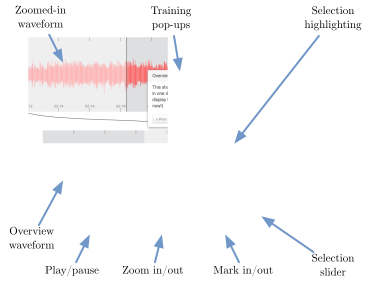
\includegraphics[width=\columnwidth]{figs/browser-audio-interface.pdf}
\caption{Screenshot of the test interface with the following features:
zoomed-in audio visualisation (1),
overview audio visualisation (2),
play/pause control (3),
zoom in/out control (4),
mark in/out buttons (5),
selection slider (6),
selection highlighting (7),
and training pop-ups (8).}
\label{fig:visualisation-interface}
\end{figure}

The interface displayed the overall visualisation as well as a zoomed in view above.  Either view could be used to
navigate the audio by clicking on it, or to adjust the segment by dragging its edge.  The participant could play/pause
the audio, control the zoom level, and mark in-- and out-points using buttons at the bottom.  Training was conducted
using a `pop-up tour', which guided the user through the interface's operation using a series of pop-up text boxes for
each feature.

%We configured the interface to log and timestamp every action the user made, including each seek, play/pause, select
%and zoom action. We also used these metrics to calculate the task completion time, defined as the time between the
%first user action and the last select action.

We generated the visualisations of the audio clips using a plugin framework we developed called `Vampeyer', which
mapped the results of an audio analysis algorithm to a bitmap image. We then integrated those images into our test
interface using in an interactive web-based audio visualisation library we developed called `BeatMap'.  Sections
\ref{sec:vampeyer} and \ref{sec:beatmap} contain more detail about Vampeyer and BeatMap, respectively.


\subsection{Procedure}

Before the study began, we asked the participant to read an informaton sheet and agree to a consent form. There were
four stages to the study:


\paragraph{Stage 1: Demographics}
We asked the participant about their gender, age and the following questions, to gauge their level of experience:

{\singlespacing
\begin{itemize}
  \item Do you understand what an audio waveform is? [Yes/No]
  \item Have you previously used any consumer audio editing software? (e.g.  Audacity, GarageBand) [Yes/No]
  \item Have you previously used any professional audio editing software? (e.g.  ProTools, Logic, Cubase/Nuendo, SADiE,
    Startrack) [Yes/No]
  \item How many years (if any) have you worked with audio in a professional capacity? [\textit{number}]
\end{itemize}
}

\paragraph{Stage 2: Training}
We used a `pop-up tour' to overlay a sequence of text boxes on the interface (see
Figure~\ref{fig:visualisation-interface}). These explained the features and operation of the test interface, then
prompted the user to complete and submit a training task. We measured the error of the training task and did not allow
the participant to continue until they had completed the task successfully.

\paragraph{Stage 3: Segmentation and task load questionnairre}
The participant used the test interface to mark the position of music in a speech recording, then submit their result.
We logged and timestamped the participant's actions, including seek, play/pause, zoom and mark.  This exercise was
repeated three times for each condition, for a total of nine tasks.  We chose to group the presentation of the
conditions rather than interleave them (e.g. AAABBBCCC instead of ACACBABCB).  We did this do we could capture feedback
directly after each condition, and to avoid possible confusion due to switching too often.

After completing the three tasks for each condition, the participant rated the workload of those tasks
using the NASA-TLX metrics. We captured the responses using sliders with the question-dependent labels on each end.

\paragraph{Stage 4: Comparison}
We asked the participant to select which condition they thought was the easiest, and which was the most frustrating,
using the thumbnail images in Figure~\ref{fig:conditions}.

\subsection{Test data}
We used radio programme clips for the audio data, by choosing a representative selection of programme formats, musical
genres and radio stations, shown in Table~\ref{tab:clips}.  We sourced the audio content from BBC recordings of
transmission (ROT). We selected five-minute clips that contained one section of music, with speech before and after. We
cut the clips so that the music was in a different position in each clip.

\begin{table}[htbp]
  \begin{center}
    {\small
    \begin{tabular}{l l l l l l}
      \hline
      \textbf{Clip} & \textbf{Network} & \textbf{Prog name} & \textbf{Prog format} & \textbf{Music genre} \\ \hline
      Training & Radio 4 & Desert Island Discs & Interview & Ambient \\
      1 & 1 Xtra & Sian Anderson & Breakfast & Dance \\
      2 & 6 Music & Lauren Laverne & Single & Indie \\
      3 & Radio 2 & Ken Bruce & Phone quiz & Lounge \\
      4 & Radio 3 & Breakfast show & Single & Classical \\
      5 & 5 Live & Sports report & Sports & Band \\
      6 & Radio 1 & Zane Lowe & Interview & Rap \\
      7 & Radio 2 & Jo Whiley & Review & Pop \\
      8 & Radio 4 & Afternoon drama & Drama & Classical \\
      9 & Radio 4 & Front Row & Interview & Alternative \\ \hline
    \end{tabular}
  }
  \end{center}
  \caption{Descriptions of the radio programmes used for the evaluation}
  \label{tab:clips}
\end{table}

Each audio clip can only be used once per participant, otherwise they would be able to remember the location of the the
music. To define a balanced sequence for the audio clips, we used a Williams design Latin square, generated using the
`crossdes' package\footnote{\url{http://cran.r-project.org/web/packages/crossdes/index.html}} in R.  We used Latin
squares to block out the effect of the order of presentation, and a Williams design, which is balanced for first-order
carryover effects.  As the sequence length is an odd number, the Williams design uses two latin squares to produce an
$18\times9$ matrix.

To generate the visualisation sequence, we needed to produce a balanced $18\times3$ matrix. We did this by taking three
columns from our $18\times9$ and mapping the values 1--3, 4--6 and 7--9 to 1, 2 and 3, respectively.  By calculating
the carryover effect of each column of the $18\times9$ matrix, we found that the middle three columns had the minimum
carryover effect, so we used them for our visualisation sequence.

%\begin{table}
%\centering
  %{\small
    %\begin{tabular}{|rrrrrrrrr|}
      %\hline
      %1 & 2 & 9 & 3 & 8 & 4 & 7 & 5 & 6 \\ 
      %3 & 3 & 3 & 2 & 2 & 2 & 1 & 1 & 1 \\ 
      %\hline
      %2 & 3 & 1 & 4 & 9 & 5 & 8 & 6 & 7 \\ 
      %1 & 1 & 1 & 3 & 3 & 3 & 2 & 2 & 2 \\ 
      %\hline
      %3 & 4 & 2 & 5 & 1 & 6 & 9 & 7 & 8 \\ 
      %2 & 2 & 2 & 1 & 1 & 1 & 3 & 3 & 3 \\ 
      %\hline
      %4 & 5 & 3 & 6 & 2 & 7 & 1 & 8 & 9 \\ 
      %3 & 3 & 3 & 2 & 2 & 2 & 1 & 1 & 1 \\ 
      %\hline
      %5 & 6 & 4 & 7 & 3 & 8 & 2 & 9 & 1 \\ 
      %1 & 1 & 1 & 3 & 3 & 3 & 2 & 2 & 2 \\ 
      %\hline
      %6 & 7 & 5 & 8 & 4 & 9 & 3 & 1 & 2 \\ 
      %2 & 2 & 2 & 1 & 1 & 1 & 3 & 3 & 3 \\ 
      %\hline
      %7 & 8 & 6 & 9 & 5 & 1 & 4 & 2 & 3 \\ 
      %3 & 3 & 3 & 2 & 2 & 2 & 1 & 1 & 1 \\ 
      %\hline
      %8 & 9 & 7 & 1 & 6 & 2 & 5 & 3 & 4 \\ 
      %1 & 1 & 1 & 3 & 3 & 3 & 2 & 2 & 2 \\ 
      %\hline
      %9 & 1 & 8 & 2 & 7 & 3 & 6 & 4 & 5 \\ 
      %2 & 2 & 2 & 1 & 1 & 1 & 3 & 3 & 3 \\ 
      %\hline
      %6 & 5 & 7 & 4 & 8 & 3 & 9 & 2 & 1 \\ 
      %1 & 1 & 1 & 2 & 2 & 2 & 3 & 3 & 3 \\ 
      %\hline
      %7 & 6 & 8 & 5 & 9 & 4 & 1 & 3 & 2 \\ 
      %2 & 2 & 2 & 3 & 3 & 3 & 1 & 1 & 1 \\ 
      %\hline
      %8 & 7 & 9 & 6 & 1 & 5 & 2 & 4 & 3 \\ 
      %3 & 3 & 3 & 1 & 1 & 1 & 2 & 2 & 2 \\ 
      %\hline
      %9 & 8 & 1 & 7 & 2 & 6 & 3 & 5 & 4 \\ 
      %1 & 1 & 1 & 2 & 2 & 2 & 3 & 3 & 3 \\ 
      %\hline
      %1 & 9 & 2 & 8 & 3 & 7 & 4 & 6 & 5 \\ 
      %2 & 2 & 2 & 3 & 3 & 3 & 1 & 1 & 1 \\ 
      %\hline
      %2 & 1 & 3 & 9 & 4 & 8 & 5 & 7 & 6 \\ 
      %3 & 3 & 3 & 1 & 1 & 1 & 2 & 2 & 2 \\ 
      %\hline
      %3 & 2 & 4 & 1 & 5 & 9 & 6 & 8 & 7 \\ 
      %1 & 1 & 1 & 2 & 2 & 2 & 3 & 3 & 3 \\ 
      %\hline
      %4 & 3 & 5 & 2 & 6 & 1 & 7 & 9 & 8 \\ 
      %2 & 2 & 2 & 3 & 3 & 3 & 1 & 1 & 1 \\ 
      %\hline
      %5 & 4 & 6 & 3 & 7 & 2 & 8 & 1 & 9 \\ 
      %3 & 3 & 3 & 1 & 1 & 1 & 2 & 2 & 2 \\ 
      %\hline
    %\end{tabular}
    %}
    %\caption{Sequence of presentation of audio clips (top) and visualisations (bottom).}
    %\label{tab:clipseq}
%\end{table}


\subsection{Analysis}
We wanted to ensure that all participants completed their tasks correctly.  To do so, we rejected any participant that
submitted a segment with an error of more than five seconds. We calculated the error as the sum of the absolute error
of the in-point and out-point.

%\begin{figure}[ht]
  %\begin{center}
    %$ |t_{in}-t_{inREF}| + |t_{out}-t_{outREF}| \leq 5 $\\[1em]
    %where $t_{in}$ and $t_{out}$ are the in- and out-points of each selection, in seconds,
    %and $t_{inREF}$ and $t_{outREF}$ are the ground truth in- and out-points of the music.
  %\end{center}
  %\caption{Acceptance criteria for the experiment}
  %\label{eq:accept}
%\end{figure}

For the TLX metrics, we used the `Raw TLX' values by excluding the second part of the measurement in which the
importance of each subscale is rated \citep{Hart2006}.  We did this to reduce the time required for data collection,
and to be able to analyse each subscale individually. We used repeated measures ANOVA to test for statistically
significant differences in the task load responses. We then used Tukey's honest significant difference (HSD) post-hoc
test to make pairwise comparisons between the visualisation for each metric.

We couldn't re-use audio clips for the tasks, so each participant only experienced a subset of the combinations of
visualisations and audio clips. This resulted in missing data, which prevented us from using from using repeated
measures ANOVA. Instead, we used a mixed model as it can account for missing values and a repeated measures design.

We used SPSS to perform a linear mixed effects analysis of the relationship between visualisation and seek actions. As
fixed effects, we entered visualisation into the model. As random effects, we had intercepts for subjects and audio
clips. Visual inspection of residual plots did not reveal any obvious deviations from homoscedasticity or normality.
$p$-values were obtained by likelihood ratio tests of the full model with the effect in question against the model
without the effect in question.

%\paragraph{Box plot}
%A box plot \citep{McGill1978} is a technique used to graph distributions by their quartile values (i.e. 25th, 50th and
%75th percentiles). An example can be seen in Figure~\ref{fig:seekbox}. The box extends from the first to the third
%quartile, with the second quartile (median) marked as a line through the box.  Lines are drawn from the box to the
%minimum and maximum, known as `whiskers', however data determined to be outliers are marked separately as crosses.  The
%95\% confidence interval of the median is marked as a notch in the box.

%\paragraph{ANOVA}
%Analysis of variance is a method of testing whether the mean values of several groups are equal or not. It assumes that
%the observations are independent, that the data have a normal distribution, and that the variance within the groups are
%similar. One-way ANOVA tests for a null hypothesis that the means values of the factors are the same.

%\paragraph{Tukey's test}
%If the null hypothesis is rejected using ANOVA, we know that there is a difference between the factors, but we don't
%know which ones. Tukey's test is a post-hoc analysis for discovering the difference between individual factors.  It
%assumes that the observations are independent and that the variance within the groups are similar.

%When Tukey's test is graphed, the mean values are represented by a dot with a line either side showing the confidence
%interval. Confidence intervals which don't overlap can be said to be significantly different.

%\paragraph{Standardisation}
%Some observations can be biased through participant behaviour. For example, person A navigates audio recordings by
%quickly clicking along the timeline while person B navigates with only a few considered clicks. To block this factor,
%the responses of each participant can be standardised so that they have a mean value of 0 and a standard deviation of
%1. This allows the difference between different participants responses to be measured fairly.

%Standardisation maps observations to the `\textbf{standard score}'. This is a dimensionless unit which represents the
%number of standard deviations an observation is above the mean.

\section{Results}
Of the 63 participants who completed the study, 41 (65\%) passed the acceptance criteria. This was lower than expected,
so we analysed the rejected tasks and participants to look for anything that might explain the high number of
rejections.

\begin{figure}[h]
\centering
  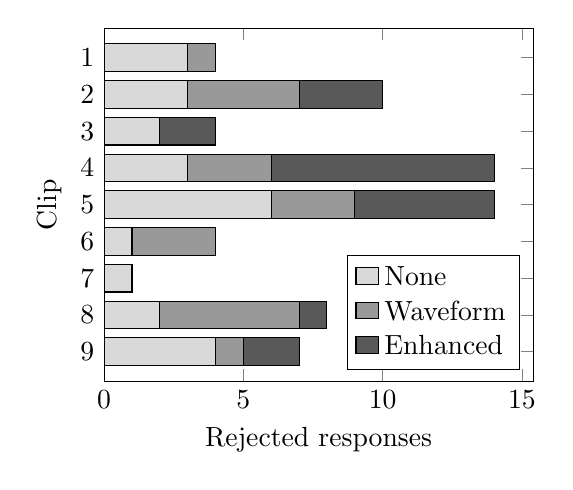
\begin{tikzpicture}
    \begin{axis}[
      height=0.5\textwidth,
      %width=0.9\textwidth,
      legend pos=south east,
      legend cell align=left,
      xbar stacked,
      ytick=data,
      xmin=0,
      ylabel=Clip,
      xlabel=Rejected responses,
      symbolic y coords={9,8,7,6,5,4,3,2,1},
    ]
    \addplot[fill=black!15] coordinates
      {(4,9) (2,8) (1,7) (1,6) (6,5) (3,4) (2,3) (3,2) (3,1)};
    \addplot[fill=black!40] coordinates
      {(1,9) (5,8) (0,7) (3,6) (3,5) (3,4) (0,3) (4,2) (1,1)};
    \addplot[fill=black!65] coordinates
      {(2,9) (1,8) (0,7) (0,6) (5,5) (8,4) (2,3) (3,2) (0,1)};
    \legend{None,Waveform,Enhanced}
    \end{axis}
  \end{tikzpicture}
  \caption{Rejected clips}
  \label{fig:rejected-clips}
\end{figure}

Figure~\ref{fig:rejected-clips} shows the number of clips and conditions that were used for the rejected responses.
Although clips 4 and 5 had a higher number of rejections, the responses came from all clips and all conditions. There
was also no combination of clips and conditions that caused an unusually high number of rejections.  We did not find
any notable difference in error between the in-points and out-points.  Figure~\ref{fig:demographics} shows the
demographics of the participants.  We did not find any correlation between rejection and DAW experience, professional
experience, age or gender.

\begin{figure}[h]
\centering
\begin{subfigure}{.5\textwidth}
  \centering
  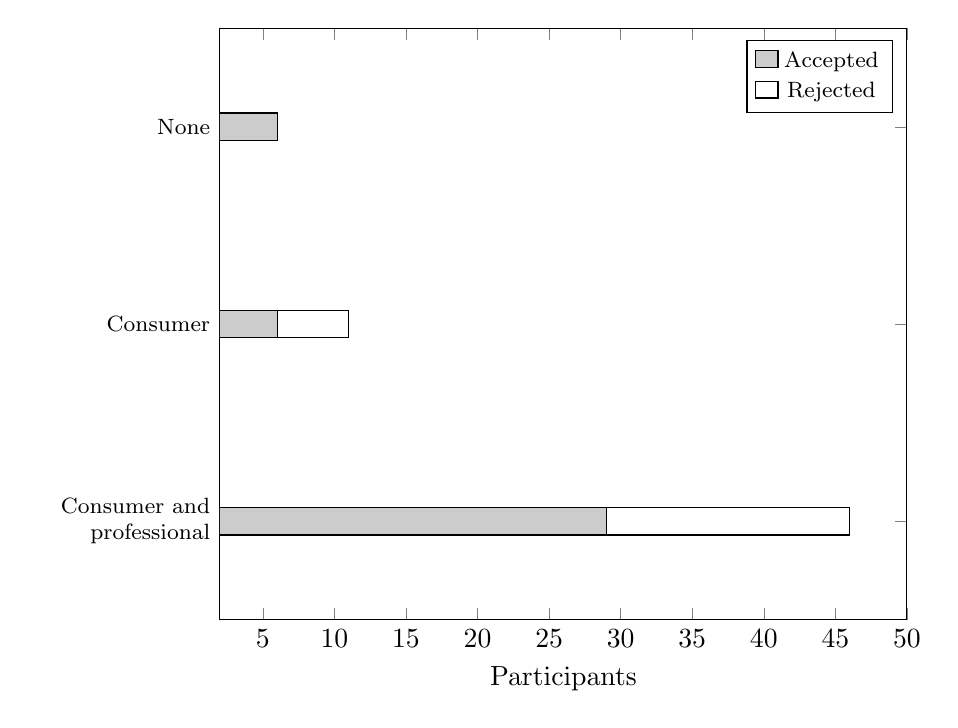
\begin{tikzpicture}
    \begin{axis}[
      height=0.75\textwidth,
      width=0.85\textwidth,
      enlarge y limits=0.25,
      xbar stacked,
      ytick=data,
      yticklabel style={font=\footnotesize,text width=2.2cm,align=right},
      xlabel=Participants,
      symbolic y coords={Consumer and professional,Consumer,None},
      legend style={font=\footnotesize},
    ]
    \addplot[fill=black!20] coordinates
      {(29,Consumer and professional) (6,Consumer) (6,None)};
    \addplot[fill=white] coordinates
      {(17,Consumer and professional) (5,Consumer) (0,None)};
    \legend{Accepted,Rejected}
    \end{axis}
  \end{tikzpicture}
  \caption{DAW experience}
  \label{fig:daw-experience}
\end{subfigure}%
\begin{subfigure}{.5\textwidth}
  \centering
  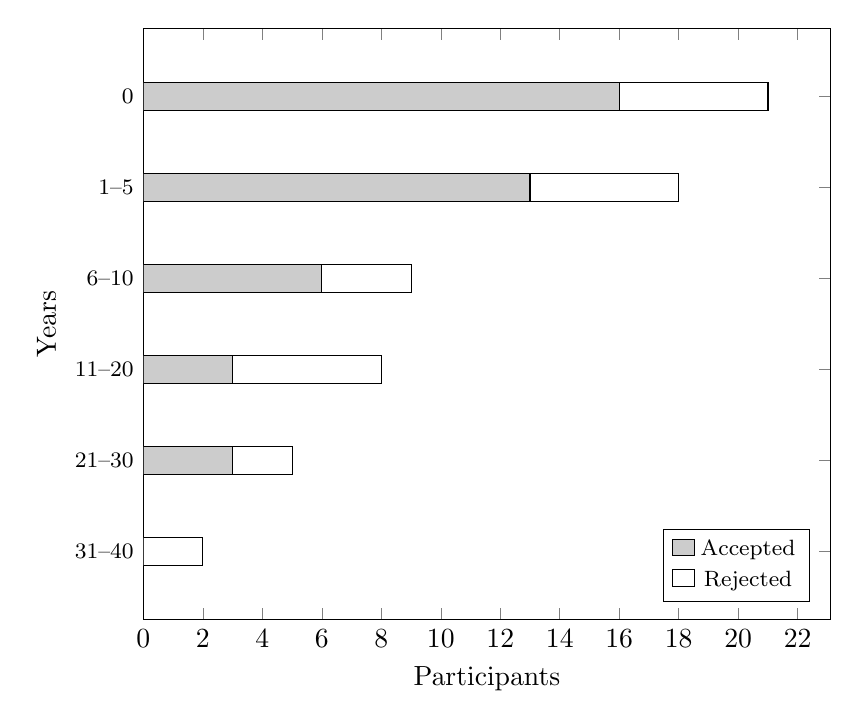
\begin{tikzpicture}
    \begin{axis}[
      height=0.75\textwidth,
      width=0.85\textwidth,
      legend pos=south east,
      enlarge y limits=0.15,
      xbar stacked,
      ytick=data,
      yticklabel style={font=\footnotesize},
      xmin=0,
      ylabel=Years,
      xlabel=Participants,
      symbolic y coords={31--40,21--30,11--20,6--10,1--5,0},
      legend style={font=\footnotesize},
    ]
    \addplot[fill=black!20] coordinates
      {(0,31--40) (3,21--30) (3,11--20) (6,6--10) (13,1--5) (16,0)};
    \addplot[fill=white] coordinates
      {(2,31--40) (2,21--30) (5,11--20) (3,6--10) (5,1--5) (5,0)};
    \legend{Accepted,Rejected}
    \end{axis}
  \end{tikzpicture}
  \caption{Professional experience}
  \label{fig:pro-experience}
\end{subfigure}
\caption{Participant demographics}
\label{fig:demographics}
\end{figure}

We were unable to find any systematic reasons for the rejected responses. However, as the test was online and
unsupervised, this may have led some participants to perform the task to a lower standard than was required.

Figure~\ref{fig:demographics} shows that the vast majority of participants had previous experience of using both
consumer and professional audio editing software. 61\% of participants also had professional experience of working with
audio. All participants reported that they understood what an audio waveform was.
%The demographic of the participants showed a heavy bias (80\%) of male participants, and a larger proportion in the
%26-45 age range (see Figure~\ref{fig:age}). This reflects the population to which the experiment was promoted (see
%Section~\ref{sec:promo}) and is not expected to skew the results.


%\begin{figure}[ht]
  %\centering
  %\includegraphics[width=0.5\textwidth]{figs/reject-daw.pdf}
  %\caption{Response of rejected participants when asked whether they had previously used consumer/professional audio
    %editing software}
  %\label{fig:rejectdaw}
%\end{figure}

%\begin{figure}[ht]
%\centering
%\begin{subfigure}{.5\textwidth}
  %\centering
  %\includegraphics[width=\linewidth]{figs/rejects-vis.pdf}
  %\caption{By visualisation}
  %\label{fig:rejectvis}
%\end{subfigure}%
%\begin{subfigure}{.5\textwidth}
  %\centering
  %\includegraphics[width=\linewidth]{figs/rejects-clip.pdf}
  %\caption{By clip}
  %\label{fig:rejectclip}
%\end{subfigure}
%\caption{Analysis of incorrect responses}
%\label{fig:rejects}
%\end{figure}

%\begin{figure}[ht]
  %\centering
  %\includegraphics[width=0.5\textwidth]{figs/age.pdf}
  %\caption{Age and gender of participants. Male/female ratio was 32/8
    %(80\%/20\%). One participant declined to respond to the question.}
  %\label{fig:age}
%\end{figure}

%\begin{figure}[ht]
%\centering
%\begin{subfigure}{.5\textwidth}
  %\centering
  %\includegraphics[width=\textwidth]{figs/daw.pdf}
  %\caption{Previous use of audio editing software}
  %\label{fig:experiencedaw}
%\end{subfigure}%
%\begin{subfigure}{.5\textwidth}
  %\centering
  %\includegraphics[width=\linewidth]{figs/experience.pdf}
  %\caption{Years of professional audio experience}
  %\label{fig:experienceyears}
%\end{subfigure}
%\caption{Response of participants to questions about experience}
%\label{fig:experience}
%\end{figure}

\subsection{Performance metrics}

We analysed the performance metrics using a linear mixed model. We configured the visualisations as a fixed effect and
the audio clips and participants as random effects.  Our model found statistically significant differences between the
three conditions for seek actions, task time, and task error.  Figure~\ref{fig:visualisation-metrics} shows the mean
values and confidence intervals of the performance metrics and Table~\ref{tab:pairwise} lists the statistical
significance of the pairwise comparisons between the conditions.

\begin{figure}[ht]
  \centering
  \begin{subfigure}[t]{0.5\textwidth}
    \centering
    \begin{tikzpicture} 
    \begin{axis}[
      width=\textwidth,
      ylabel=Seek actions (count),
      xtick={1,2,3},
      xticklabels={None,Waveform,Enhanced}]
      \addplot[black,mark=*]
        plot[error bars/.cd, y dir=both, y explicit]
        coordinates {
          (1, 29.5) +- (3.7,3.7)
          (2, 24.3) +- (3.6,3.6)
          (3, 16.8) +- (3.1,3.1)
        };
    \end{axis} 
    \end{tikzpicture}
    \caption{Seek actions}
  \end{subfigure}%
  ~
  \begin{subfigure}[t]{0.5\textwidth}
    \centering
    \begin{tikzpicture} 
    \begin{axis}[
      width=\textwidth,
      ylabel=Task error (seconds),
      xtick={1,2,3},
      xticklabels={None,Waveform,Enhanced}]
      \addplot[black,mark=*]
        plot[error bars/.cd, y dir=both, y explicit]
        coordinates {
          (1, 0.645) +- (0.121,0.121)
          (2, 0.610) +- (0.121,0.121)
          (3, 0.523) +- (0.109,0.109)
        };
    \end{axis} 
    \end{tikzpicture}
    \caption{Task error}
  \end{subfigure}

  \begin{subfigure}[t]{0.5\textwidth}
    \centering
    \begin{tikzpicture} 
    \begin{axis}[
      width=\textwidth,
      ylabel=Task time (seconds),
      xtick={1,2,3},
      xticklabels={None,Waveform,Enhanced}]
      \addplot[black,mark=*]
        plot[error bars/.cd, y dir=both, y explicit]
        coordinates {
          (1, 70.6) +- (16.76,16.76)
          (2, 68.7) +- (16.49,16.49)
          (3, 59.7) +- (16.47,16.47)
        };
    \end{axis} 
    \end{tikzpicture}
    \caption{Task time}
  \end{subfigure}
  \caption{Mean performance metric values with 95\% confidence intervals}
  \label{fig:visualisation-metrics}
\end{figure}

\definecolor{lightred}{RGB}{255,204,204}
\definecolor{lightamber}{RGB}{255,204,153}
\definecolor{lightgreen}{RGB}{204,255,204}
\newcommand{\highsig}{\cellcolor{black!20}}
\newcommand{\medsig}{\cellcolor{black!10}}
\newcommand{\nosig}{\cellcolor{white}}
\begin{table}[ht]
  %\footnotesize
  \begin{threeparttable}
%\resizebox{\textwidth}{!}{
    \begin{tabular}{L{.35\textwidth-2\tabcolsep} C{.21\textwidth-2\tabcolsep} C{.21\textwidth-2\tabcolsep} C{.23\textwidth-2\tabcolsep}}
\hline
& \textbf{None vs Waveform} & \textbf{None vs Enhanced} & \textbf{Waveform vs Enhanced} \\ \hline
	Seek actions        & \highsig$<0.01$ & \highsig$<0.01$ & \highsig$<0.01$ \\
	Task error          & \nosig$>0.05$ & \highsig$<0.01$ & \medsig$<0.05$ \\
	Task time           & \nosig$>0.05$ & \highsig$<0.01$ & \highsig$<0.01$ \\
  TLX Effort\tnote{1} & \medsig$<0.05$ & \highsig$<0.01$ & \highsig$<0.01$ \\
	TLX Frustration     & \medsig$<0.05$ & \highsig$<0.01$ & \medsig$<0.05$ \\
	TLX Mental demand   & \nosig$>0.05$ & \highsig$<0.01$ & \highsig$<0.01$ \\
	TLX Performance     & \nosig$>0.05$ & \highsig$<0.01$ & \medsig$<0.05$ \\
	TLX Physical demand & \nosig$>0.05$ & \highsig$<0.01$ & \highsig$<0.01$ \\
  TLX Temporal demand\tnote{1} & \nosig$>0.05$ & \nosig$>0.05$ & \medsig$<0.05$ \\ \hline
\end{tabular}
\caption{$p$-values of pairwise comparisons}
\label{tab:pairwise}
\begin{tablenotes}
    \item[1] Mauchly's Test of Sphericity indicated that the assumption of sphericity had been violated for the effort
      metric [$\chi^2(2) = 9.657, p=.008$] and temporal demand metric [$\chi^2(2) = 17.918, p<.001$]. Therefore, we
      have adjusted the degrees of freedom for the univariate tests using the conservative Greenhouse-Geisser
      Correction.
  \end{tablenotes}
%}
  \end{threeparttable}
\end{table}


\subsubsection{Seek actions}
The audio visualisation had a significant effect on the number of seek actions used to complete the task
[$F(3,366)=93.871, p<.00001$]. On average, the enhanced waveform required 7.5 (30\%) fewer seek actions than the
normal waveform, and 12.7 (43\%) fewer than having no visualisation. Additionally, the normal waveform required 5.2
(17\%) fewer seek actions than having no visualisation. The difference in seek actions between all three conditions
were statistically significant ($p<.01$).

\subsubsection{Task time}
The audio visualisation had a significant effect on the time required to complete the task [$F(3,366)=25.261,
p<.00001$].  On average, the task was completed 9 seconds (13\%) faster using the enhanced waveform compared to the
normal waveform ($p<.01$), and 10.9 seconds (15\%) faster compared to having no visualisation ($p<.01$). There was no
statistically significant difference in task completion time between the normal waveform and no visualisation. 

\subsubsection{Task error}
The audio visualisation had a significant effect on the accuracy of the task result [$F(3,366)=42.462, p<.00001$].  On
average, the error when using the enhanced waveform was 87ms (14\%) lower than when using the normal waveform
($p<.05$), and 122ms (19\%) lower than when there was no visualisation ($p<.01$). There was no statistically
significant difference in task error between the normal waveform and no visualisation.

%\begin{figure}[ht] \centering \begin{subfigure}{.5\textwidth} \centering
%\includegraphics[width=\textwidth]{figs/seek-std.pdf} \caption{Box plot} \label{fig:seekbox} \end{subfigure}%
%\begin{subfigure}{.5\textwidth} \centering \includegraphics[width=\linewidth]{figs/seek-std-tukey99.pdf}
%\caption{Tukey's test (99\% confidence interval)} \label{fig:seektukey} \end{subfigure} \caption{Number of seek
%actions, standardised per participant} \label{fig:seek} \end{figure}

%\begin{figure}[ht] \centering \begin{subfigure}{.5\textwidth} \centering
%\includegraphics[width=\textwidth]{figs/playstart-to-selectend-std.pdf} \caption{Box plot} \label{fig:selecttimebox}
%\end{subfigure}% \begin{subfigure}{.5\textwidth} \centering
%\includegraphics[width=\linewidth]{figs/playstart-to-selectend-std-tukey95.pdf} \caption{Tukey's test (95\% confidence
%interval)} \label{fig:selecttimetukey} \end{subfigure} \caption{Selection time (time between start of playback and
%final selection), standardised per participant} \label{fig:selecttime} \end{figure}

%\begin{figure}[ht]
%\centering
%\begin{subfigure}{.5\textwidth}
  %\centering
  %\includegraphics[width=\textwidth]{figs/outpoint-abserr.pdf}
  %\caption{Box plot}
  %\label{fig:outpointerrbox}
%\end{subfigure}%
%\begin{subfigure}{.5\textwidth}
  %\centering
  %\includegraphics[width=\linewidth]{figs/outpoint-abserr-tukey95.pdf}
  %\caption{Tukey's test (95\% confidence interval)}
  %\label{fig:outpointerrtukey}
%\end{subfigure}
%\caption{Absolute error for the outpoint of selections}
%\label{fig:outpointerr}
%\end{figure}

%\paragraph{Zoom}
%The experimental interface included two displays -- one overview display covering the length of the recording, and a
%zoomed display which showed a magnified part of that. The number of times the zoom in and zoom out buttons were pressed
%was logged. The sum of these values for each visualization is shown in Figure~\ref{fig:zoomtotal}. By subtracting zoom
%out from zoom in, we can infer what the final zoom level was when the response was submitted. The final zoom levels for
%each visualization are shown in Figure~\ref{fig:zoomfinal}.

%\begin{figure}[h!]
%\centering
%\begin{subfigure}{.5\textwidth}
  %\centering
  %\includegraphics[width=\linewidth]{figs/zoomtotal.pdf}
  %\caption{Total zoom actions}
  %\label{fig:zoomtotal}
%\end{subfigure}%
%\begin{subfigure}{.5\textwidth}
  %\centering
  %\includegraphics[width=\linewidth]{figs/zoomfinal.pdf}
  %\caption{Final zoom level}
  %\label{fig:zoomfinal}
%\end{subfigure}
%\caption{Analysis of zoom usage}
%\label{fig:zoom}
%\end{figure}

%Most of the time, participants didn't touch the zoom controls and opted to leave it on the default x5 zoom level, which
%displays roughly one minute of audio across 1045 pixels ($\sim$50ms per pixel). Other than the x5 level, x15 was more
%popular than x10 for all visualizations and x20 was barely used at all.

\subsection{Task load ratings}

We analysed the task load ratings using repeated measures multivariate ANOVA, which found that the audio visualisation
had a significant effect on the number of task load ratings from participants [$F(12,152)=3.552, p<0.001$].
Figure~\ref{fig:tlx-results} shows the mean values and confidence intervals of the task load metrics and
Table~\ref{tab:pairwise} lists the statistical significance of the pairwise comparisons between the conditions.


Participants reported that compared to both the normal waveform and no visualisation, the enhanced waveform was less
mentally and physically demanding, had better performance, was less frustrating and required less effort.  They also
rated the enhanced waveform as less temporally demanding than the normal waveform. Compared to having no visualisation,
participants rated the normal waveform as being less frustrating and requiring less effort. 

\begin{figure}[p]
  \centering
  \begin{subfigure}[t]{0.5\textwidth}
    \centering
    \begin{tikzpicture} 
    \begin{axis}[
      width=\textwidth,
      ylabel=Effort,
      xtick={1,2,3},
      xticklabels={None,Waveform,Enhanced}]
      \addplot[black,mark=*]
        plot[error bars/.cd, y dir=both, y explicit]
        coordinates {
          (1, -0.122) +- (1.49,1.49)
          (2, -2.244) +- (1.51,1.51)
          (3, -4.220) +- (1.28,1.28)
        };
    \end{axis} 
    \end{tikzpicture}
    \caption{Effort}
  \end{subfigure}%
  ~
  \begin{subfigure}[t]{0.5\textwidth}
    \centering
    \begin{tikzpicture} 
    \begin{axis}[
      width=\textwidth,
      ylabel=Frustration,
      xtick={1,2,3},
      xticklabels={None,Waveform,Enhanced}]
      \addplot[black,mark=*]
        plot[error bars/.cd, y dir=both, y explicit]
        coordinates {
          (1, -0.829) +- (2.03,2.03)
          (2, -2.976) +- (1.67,1.67)
          (3, -5.268) +- (1.24,1.24)
        };
    \end{axis} 
    \end{tikzpicture}
    \caption{Frustration}
  \end{subfigure}%

  \begin{subfigure}[t]{0.5\textwidth}
    \centering
    \begin{tikzpicture} 
    \begin{axis}[
      width=\textwidth,
      ylabel=Mental demand,
      xtick={1,2,3},
      xticklabels={None,Waveform,Enhanced}]
      \addplot[black,mark=*]
        plot[error bars/.cd, y dir=both, y explicit]
        coordinates {
          (1, -1.390) +- (1.68,1.68)
          (2, -2.585) +- (1.45,1.45)
          (3, -4.585) +- (1.23,1.23)
        };
    \end{axis} 
    \end{tikzpicture}
    \caption{Mental demand}
  \end{subfigure}%
  ~
  \begin{subfigure}[t]{0.5\textwidth}
    \centering
    \begin{tikzpicture} 
    \begin{axis}[
      width=\textwidth,
      ylabel=Performance,
      xtick={1,2,3},
      xticklabels={None,Waveform,Enhanced}]
      \addplot[black,mark=*]
        plot[error bars/.cd, y dir=both, y explicit]
        coordinates {
          (1, -5.415) +- (1.10,1.10)
          (2, -6.317) +- (1.11,1.11)
          (3, -7.341) +- (0.88,0.88)
        };
    \end{axis} 
    \end{tikzpicture}
    \caption{Performance}
  \end{subfigure}%

  \begin{subfigure}[t]{0.5\textwidth}
    \centering
    \begin{tikzpicture} 
    \begin{axis}[
      width=\textwidth,
      ylabel=Physical demand,
      xtick={1,2,3},
      xticklabels={None,Waveform,Enhanced}]
      \addplot[black,mark=*]
        plot[error bars/.cd, y dir=both, y explicit]
        coordinates {
          (1, -3.122) +- (1.81,1.81)
          (2, -4.098) +- (1.45,1.45)
          (3, -6.171) +- (1.08,1.08)
        };
    \end{axis} 
    \end{tikzpicture}
    \caption{Physical demand}
  \end{subfigure}%
  ~
  \begin{subfigure}[t]{0.5\textwidth}
    \centering
    \begin{tikzpicture} 
    \begin{axis}[
      width=\textwidth,
      ylabel=Temporal demand,
      xtick={1,2,3},
      xticklabels={None,Waveform,Enhanced}]
      \addplot[black,mark=*]
        plot[error bars/.cd, y dir=both, y explicit]
        coordinates {
          (1, -3.171) +- (1.75,1.75)
          (2, -3.268) +- (1.51,1.51)
          (3, -4.878) +- (1.39,1.39)
        };
    \end{axis} 
    \end{tikzpicture}
    \caption{Temporal demand}
  \end{subfigure}%
  \caption{Mean TLX values with 95\% confidence intervals}
  \label{fig:tlx-results}
\end{figure}

%\begin{figure}[p]
  %\centering
  %\includegraphics[width=\textwidth]{figs/tlx-std.pdf}
  %\caption{Standard score of NASA Task Load Index responses for each visualization, standardised per participant.}
  %\label{fig:tlx}
%\end{figure}

%\begin{figure}[p]
  %\centering
  %\includegraphics[width=\textwidth]{figs/tlx-std-tukey95.pdf}
  %\caption{Standard score of NASA Task Load Index responses for each visualization, standardised per participant.}
  %\label{fig:tlxtukey}
%\end{figure}

\subsection{Comparison}
Participants were asked to select which audio visualisation was the easiest to use, and which was the most frustrating.
The results are shown in Figure~\ref{fig:visualisation-comparison}.  The enhanced waveform was rated as the easiest
audio visualisation to use by 76\% of the participants.  Having no visualisation was rated as the most frustrating
condition by two-thirds of the participants. The normal waveform was not considered by many to be the easiest, nor the
most frustrating.

\begin{figure}[ht]
\centering
\begin{subfigure}{.5\textwidth}
  \centering
  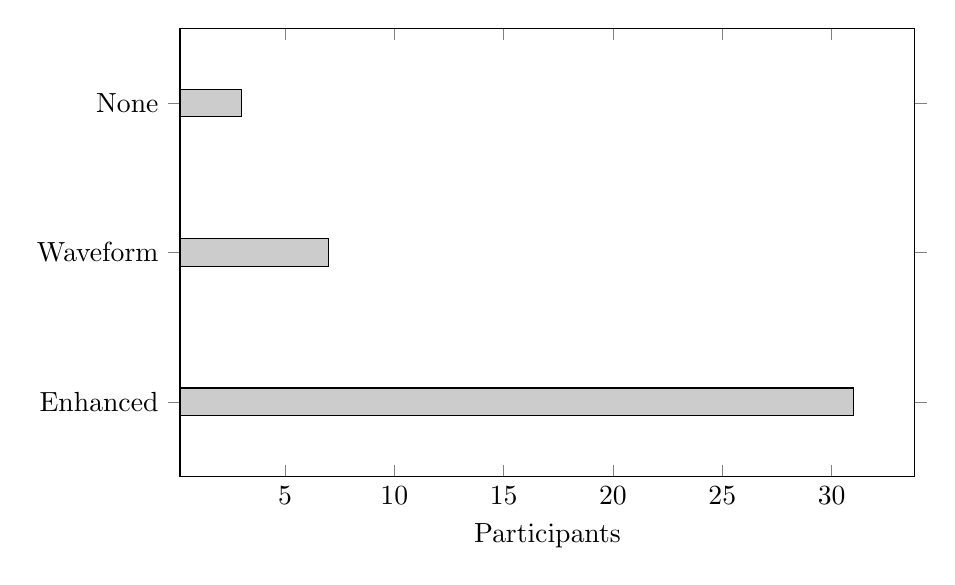
\begin{tikzpicture}
    \begin{axis}[
      height=0.6\textwidth,
      width=0.9\textwidth,
      %xmin=0,
      %xmax=38,
      enlarge y limits=0.25,
      xbar,
      ytick=data,
      xlabel=Participants,
      symbolic y coords={Enhanced,Waveform,None},
      %nodes near coords, nodes near coords align={horizontal},
    ]
    \addplot[fill=black!20] coordinates
      {(31,Enhanced) (7,Waveform) (3,None)};
    \end{axis}
  \end{tikzpicture}
  \caption{Easiest}
  \label{fig:easiest}
\end{subfigure}%
\begin{subfigure}{.5\textwidth}
  \centering
  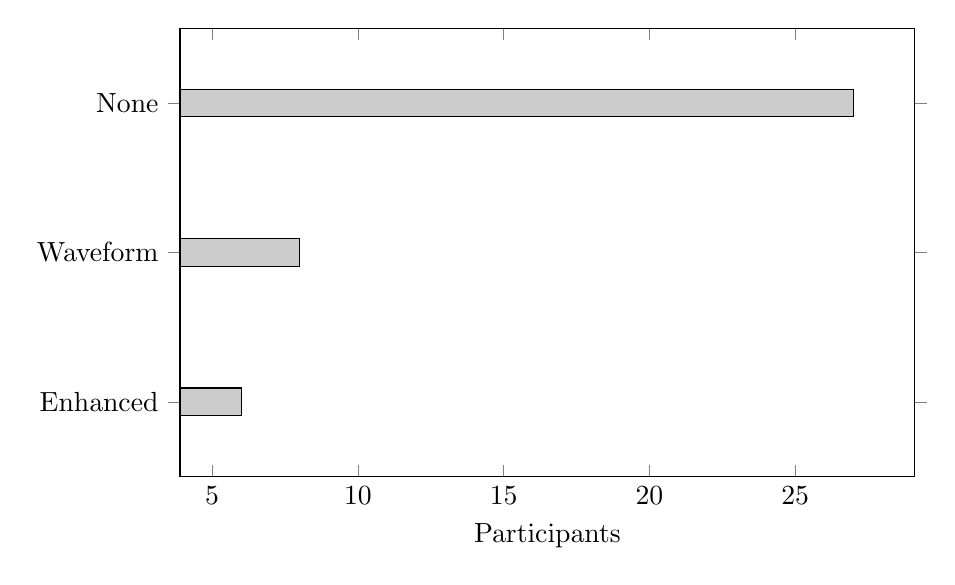
\begin{tikzpicture}
    \begin{axis}[
      height=0.6\textwidth,
      width=0.9\textwidth,
      %xmin=0,
      %xmax=32,
      enlarge y limits=0.25,
      xbar,
      ytick=data,
      xlabel=Participants,
      symbolic y coords={Enhanced,Waveform,None},
      %nodes near coords, nodes near coords align={horizontal},
    ]
    \addplot[fill=black!20] coordinates
      {(6,Enhanced) (8,Waveform) (27,None)};
    \end{axis}
  \end{tikzpicture}
  \caption{Most frustrating}
  \label{fig:frustrating}
\end{subfigure}
\caption{Preferences of participants}
\label{fig:visualisation-comparison}
\end{figure}

\subsection{Hypotheses}



\begin{table}[h]
  \centering
  \begin{tabular}{l c c}
    \hline
                  & C1 $<$ C2           & C2 $<$ C3 \\
    \hline
    H1 (effort)   & \textbf{Confirmed}  & \textbf{Confirmed} \\
    H2 (time)     & Unconfirmed         & \textbf{Confirmed} \\
    H3 (accuracy) & Unconfirmed         & \textbf{Confirmed} \\
    \hline
  \end{tabular}
  \caption{Summary of hypothesis testing}
  \label{tab:hypotheses}
\end{table}


%\begin{figure}[ht]
%\centering
%\begin{subfigure}{.5\textwidth}
  %\centering
  %\includegraphics[width=\textwidth]{figs/easiest.pdf}
  %\caption{Easiest to use}
  %\label{fig:easiest}
%\end{subfigure}%
%\begin{subfigure}{.5\textwidth}
  %\centering
  %\includegraphics[width=\linewidth]{figs/frustrating.pdf}
  %\caption{Most frustrating}
  %\label{fig:frustrating}
%\end{subfigure}
%\caption{Response of participants when asked to compare the visualisations
  %using different criteria}
%\label{fig:compare}
%\end{figure}

%\subsection{Interaction behaviour}
%This section looks at how participants used the features available in the online audio interface, full described in
%Section~\ref{sec:iface}.
%Informal observation of some participants as they completed the experiment
%revealed that some people used the interface in different ways. For example,
%when one participant had completed their selection, they scanned through the
%remaining unselected content to check that there were no other pieces of music.

%\begin{figure}[ht]
%\centering
%\begin{subfigure}{.5\textwidth}
  %\centering
  %\includegraphics[width=\linewidth]{figs/top-v-bot-pref.pdf}
  %\caption{Display}
  %\label{fig:displaypref}
%\end{subfigure}%
%\begin{subfigure}{.5\textwidth}
  %\centering
  %\includegraphics[width=\linewidth]{figs/mark-v-slide-pref.pdf}
  %\caption{Selection method}
  %\label{fig:selectpref}
%\end{subfigure}
%\caption{Preference of participants}
%\label{fig:pref}
%\end{figure}

%\paragraph{Top/bottom display}
%There are two displays that make up the interface -- a zoomed display at the top and an overview display on the bottom.
%Either of the displays can be used to navigate the recording and make selections.

%For each participant, the number of tasks where they used the zoom display more than the overview (and vice-versa) were
%counted. Figure~\ref{fig:displaypref} shows number of participants who, on average, used the zoomed or overview display
%more.

%The results show a clear preference for using the overview display more than the zoom display. Coupled with the results
%of zoom usage in Section~\ref{sec:studymetrics}, we can see that for this task most people opted just to work in the
%overview display, despite only having a resolution of roughly 300ms per pixel.

%An analysis of the overview and zoom display's usage between different visualization methods did not find any notable
%difference.

%\paragraph{Selection method}
%The design of the interface gave participants two methods of making a selection -- buttons to mark in and out points
%using the cursor, and a slider where the in and out points could be dragged around. The cursor can be moved around in
%both the overview and zoomed displays, whereas the slider is only available at the x1 zoom level. This makes the
%buttons more useful for fine edits, where high precision is needed. When using the slider, the selection display
%updates as you move it making it easier for people to see where their selection is.

%For each response, the method with the most actions was found and these preferences were summed for each participant to
%calculate their overall preference. The results are shown in Figure~\ref{fig:selectpref}.

%The buttons were the most popular method of making a selection, with only 17\% of people using the slider more.
%Informal feedback found that some people has a strong preference for using the slider but were frustrated that there
%wasn't a second slider available on the zoomed display.

%\section{Results}
%63 responses were received in the three weeks the experiment ran. 35\% of participants were rejected, which was higher
%than expected. An analysis of the rejected participants found that none had experience of using professional audio
%editing software, which suggests that the errors could be due to lack of experience with audio interfaces.

%The demographic of accepted participants reflected the population which was recruited: 80\% male with a larger
%proportion in the 26-45 age range. This imbalance is not expected to affect the result. Two-thirds of accepted
%participants had experience of using professional audio editing software, with the remaining participants having
%consumer-level experience or less. 39\% reported having no professional experience with audio.

%Figure~\ref{fig:seekpdf} shows the distribution of the number of seek actions for each visualization. On average, the
%number of seek actions required to select the music is lowest for the enhanced waveform and highest for no waveform.
%However, individual participants had different styles of interaction; for example, some people had a tendency to seek
%around a lot whereas others didn't. In order to account for this, the performance and TLX metrics were standardised for
%each participant.

%\begin{figure}[!h]
%\centering
%\includegraphics[width=0.6\columnwidth]{figs/seek-pdf.pdf}
%\caption{Probability density function of number of seek actions for each
%visualization}
%\label{fig:seekpdf}
%\end{figure}

%For each metric, the standardisation function (see Equation~\ref{eq:standard}) subtracts the mean of the participant's
%scores and divides by the standard deviation. This maps observations to the `standard score', which is a dimensionless
%unit that represents the number of standard deviations an observation is above the mean.

%\begin{equation}
%std(x) = \frac{x - \mu_{part}}{\highsigma_{part}}
%\label{eq:standard}
%\end{equation}

%The performance and TLX metrics of the 41 accepted participants were analysed using ANOVA.  Significant results were
%found for the number of seek actions ($F_{2,40}=30, p<0.001$) and the selection time ($F_{2,40}=3.2,p\medsig$<0.05$$).  Tukey's
%test shows that the enhanced waveform required fewer seek actions than the normal waveform, and the normal waveform
%required fewer than no waveform (see Figure~\ref{fig:tukeyseekselect}). The selection time was shorter for the enhanced
%waveform compared to no waveform, but the normal waveform was not significantly different.

%\begin{figure}[!h]
%\centering
%\includegraphics[width=\columnwidth]{figs/seek-select.pdf}
%\caption{Tukey's test for mean number of seek actions and mean selection time}
%\label{fig:tukeyseekselect}
%\end{figure}

%Significant results were found for each of the NASA-TLX metrics ($F_{2,40}>4.8,p\highsig$<0.01$$). The normal waveform performed
%better than no waveform for mental demand, performance, effort and frustration (see Figure~\ref{fig:tlx}). The enhanced
%waveform performed better than the normal waveform for mental, physical and temporal demand, performance and effort.

%\begin{figure}[!h]
%\centering
%\includegraphics[width=\columnwidth]{figs/tlx-std-tukey95.pdf}
%\caption{Tukey's test for mean of NASA-TLX metrics (95\% CI). Lower is
  %better.}
%\label{fig:tlx}
%\end{figure}

%76\% of participants thought that the enhanced waveform was the easiest to use with the normal waveform scoring 17\%.
%Two-thirds thought that having no waveform was the most frustrating condition with 20\% choosing the normal waveform.

\section{Discussion}



\section{Conclusion}
The normal waveform required fewer seek actions than nothing but was not significantly faster. It scored better than
nothing for mental demand, performance and frustration.

The enhanced waveform required fewer seek actions than the normal waveform and was significantly faster than nothing.
It performed better than the normal waveform for mental demand, performance and effort.

%This experiment used a browser-based audio interface to conduct a within-subjects online study of how users performed
%in finding and selecting music with different audio waveforms. Three conditions were tested -- no waveform, a normal
%waveform and a waveform that was colourised using a simple speech/music discriminator.

%Compared to no waveform, the normal waveform required fewer seek actions and was rated better in terms of mental
%demand, performance, effort and frustration. Finding and selecting music with the colourised version took less time
%than with no waveform. Compared to the normal waveform, it required fewer seek actions and was rated better in terms of
%mental, physical and temporal demand, performance and effort.

%\subsection{Further work}
%The results indicate that the waveform can be significantly improved, even with a simple enhancement. The next stages
%of this research will focus on development of audio analysis and visualization algorithms/tools that address the needs
%of people working in radio production. This will be followed by an analysis of the real-world benefit of using these
%new tools.
